\documentclass[conference]{IEEEtran}
\synctex=1

%=================================================================
% 
\newcount\DraftStatus  % 0 suppresses notes to selves in text
\DraftStatus=1   % TODO: set to 0 for final version
%=================================================================
\usepackage{comment}
%=================================================================
%
\excludecomment{JournalOnly}  
\includecomment{ConferenceOnly}  
\excludecomment{TulipStyle}
%
%=================================================================
%=================================================================
% gitlatexdiff
%
%  https://gitlab.com/git-latexdiff/git-latexdiff
%=================================================================
%  git latexdiff HEAD  HEAD~5 --main templatex.tex
%  git latexdiff HEAD~1  --main templatex.tex
%  View pdf to see difference
%
%=================================================================
%
% Todo Notes for marginal comments
% 
%\newcount\DraftStatus  % 0 suppresses notes to selves in text
%\DraftStatus=1   % TODO: set to 0 for final version
\ifnum\DraftStatus=1
	\usepackage[draft,colorinlistoftodos,color=orange!30]{todonotes}
\else
	\usepackage[disable,colorinlistoftodos,color=blue!30]{todonotes}
\fi 
%\usepackage[disable]{todonotes} % notes not showed
%\usepackage[draft]{todonotes}   % notes showed
%
\makeatletter
 \providecommand\@dotsep{5}
 \def\listtodoname{List of Todos}
 \def\listoftodos{\@starttoc{tdo}\listtodoname}
 \makeatother
%
%=================================================================
%
\usepackage{color}
\newcommand{\draftnote}[3]{ 
	\todo[author=#2,color=#1!30,size=\footnotesize]{\textsf{#3}}	}
% TODO: add yourself here:
%
\newcommand{\gangli}[1]{\draftnote{blue}{GLi:}{#1}}
\newcommand{\qwu}[1]{\draftnote{red}{QWu:}{#1}}
\newcommand{\gliMarker}
	{\todo[author=GLi,size=\tiny,inline,color=blue!40]
	{Gang Li has worked up to here.}}
\newcommand{\qwuMarker}
	{\todo[author=QWu,size=\tiny,inline,color=red!40]
	{Qiong Wu has worked up to here.}}
%=================================================================

%=================================================================
%
% general packages
%  https://en.wikibooks.org/wiki/Category:Book:LaTeX
%  https://en.wikibooks.org/wiki/LaTeX/Package_Reference
%
%=================================================================
\usepackage{graphicx}
\graphicspath{{./figures/}{./graphics/}{./graphics/logos/}}

\usepackage{algorithm}
\usepackage{algorithmic}
\usepackage{breqn}
\usepackage{subcaption}
\usepackage{multirow}
\usepackage{psfrag}
\usepackage{url}
\usepackage[colorlinks,citecolor=blue]{hyperref}
%\usepackage{hyperref}
%\usepackage[colorlinks]{hyperref}
%\usepackage{cite}
\usepackage{cleveref}
\usepackage{booktabs}
\usepackage{rotating}
\usepackage{colortbl}
\usepackage{paralist}
%\usepackage{geometry}
\usepackage{epstopdf}
\usepackage{nag}
\usepackage{microtype}
\usepackage{siunitx}
\usepackage{nicefrac}
%\usepackage{breakurl}
\usepackage{fontawesome}
\usepackage{xcolor}
\usepackage{multicol}
\usepackage{wrapfig}
\usepackage{todonotes}
\usepackage{tablefootnote}
\usepackage{threeparttable}
% \usepackage{bibunits} 
% for random text
\usepackage{cite}
\usepackage{lipsum}
\usepackage[english]{babel}
\usepackage[pangram]{blindtext}
% for tikz figures
\usepackage{tikz}
\usetikzlibrary{fit,positioning,arrows.meta,shapes,arrows}
%\tikzset{neuron/.style={circle,thick,fill=black!25,minimum size=17pt,inner sep=0pt},
%	input neuron/.style={neuron, draw,thick, fill=gray!30},
%	hidden neuron/.style={neuron,fill=white,draw},
%	hoz/.style={rotate=-90}}
%
%=================================================================



\begin{TulipStyle}
\usepackage[numbers]{natbib}
%=================================================================
%
% Version control information
%
%=================================================================
\usepackage{gitinfo2}
%=================================================================
\usepackage{fancyhdr}
\pagestyle{fancy}
\fancyhead{} % clear all header fields
\fancyhead[RO,LE]{\textsl{\rightmark}}
\fancyhead[LO,RE]{\ensuremath{\Rightarrow}
		\textbf{\textbf{[CONFIDENTIAL]}}\ensuremath{\Leftarrow}}
\fancyhead[CO,CE]{}
%=================================================================
\fancyfoot{} % clear all footer fields
\fancyfoot[CE,CO]{\textbf{\thepage}} 
\fancyfoot[LO,LE]{
\includegraphics[height=.9\headheight]
{./graphics/logos/tulip-logo.eps}
		\gitVtagn-\gitBranch\ (\gitCommitterDate)}
\fancyfoot[RO,RE]{Committed by: \textsl{\gitCommitterName}}

\setlength{\headheight}{12pt}
\renewcommand{\headrulewidth}{0.4pt}
\renewcommand{\footrulewidth}{0.4pt}
%=================================================================


%=================================================================
% for math notations
% ----------------------------------------------------------------
\usepackage{mathtools}
\usepackage{amsthm}
%
% THEOREMS -------------------------------------------------------
%
\newtheorem{thm}{Theorem}[section]
\newtheorem{cor}[thm]{Corollary}
\newtheorem{lem}[thm]{Lemma}
\newtheorem{prop}[thm]{Proposition}
\theoremstyle{definition}
\newtheorem{defn}[thm]{Definition}
\theoremstyle{remark}
\newtheorem{rem}[thm]{Remark}
\numberwithin{equation}{section}
% MATH -----------------------------------------------------------
\newcommand{\norm}[1]{\left\Vert#1\right\Vert}
\newcommand{\abs}[1]{\left\vert#1\right\vert}
\newcommand{\set}[1]{\left\{#1\right\}}
\newcommand{\Real}{\mathbb R}
\newcommand{\eps}{\varepsilon}
\newcommand{\To}{\longrightarrow}
\newcommand{\BX}{\mathbf{B}(X)}
% ----------------------------------------------------------------
\newcommand{\I}{{\cal I}}
\newcommand{\Id}{{\cal I} }
\newcommand{\Dc}{{\cal D}}
\newcommand{\J}{{\cal J}}
\newcommand{\Dn}{{\cal D}_n}
\newcommand{\Dd}{{\cal D}_n }
\renewcommand{\P}{{\cal P}}
\newcommand{\Nu}{{\cal N} }
\newcommand{\B}{{\cal B}}
\newcommand{\Bf}{{\bf B}}
\newcommand{\Y}{{\bf Y}}
\newcommand{\A}{{\cal A}}
% ----------------------------------------------------------------
\newcommand{\V}{{\cal V}}
\newcommand{\M}{{\cal M}}
\newcommand{\F}{{\cal F}}
\newcommand{\Fd}{{\cal F}}
\newcommand{\BF}{{\cal BF}_n}
\newcommand{\BFd}{{\cal BF}_n}
\newcommand{\TF}{{\cal TF}_n}
\newcommand{\TFd}{{\cal TF}_n}
%\newcommand{\G}{{\cal G}}
\newcommand{\X}{{\cal X}}
\newcommand{\E}{{\cal E}}
\newcommand{\K}{{\cal K}}
\newcommand{\T}{{\cal T}_n}
\renewcommand{\H}{{\cal H}}
% ----------------------------------------------------------------
\newtheorem{Remark}{Remark}
\newtheorem{proposition}{Proposition}
\newtheorem{theorem}{Theorem}
\newtheorem{lemma}{Lemma}
\newtheorem{corollary}{Corollary}
\newtheorem{example}{Example}
\newtheorem{definition}{Definition}
\newtheorem{Algorithms}{Algorithm}
% ----------------------------------------------------------------
\newcommand{\bu}{{\mathbf 1} }
\newcommand{\bo}{{\mathbf 0} }
\newcommand{\N}{\mbox{{\sl l}}\!\mbox{{\sl N}}}
% ----------------------------------------------------------------
\def\uint{[0,1]}
\def\proof{{\scshape Proof}. \ignorespaces}
\def\endproof{{\hfill \vbox{\hrule\hbox{%
   \vrule height1.3ex\hskip1.0ex\vrule}\hrule
  }}\par}
%
%=================================================================

\hypersetup
{
    pdfauthor={\gitAuthorName},
    pdfsubject={TULIP Lab},
    pdftitle={},
    pdfkeywords={TULIP Lab, Data Science},
%	bookmarks=true,  
}

\end{TulipStyle}




\IEEEoverridecommandlockouts
% The preceding line is only needed to identify funding in the first footnote. If that is unneeded, please comment it out.
%\usepackage{amsmath,amssymb,amsfonts}
%\usepackage{algorithmic}
%\usepackage{graphicx}
%\usepackage{textcomp}
%\usepackage{xcolor}
\def\BibTeX{{\rm B\kern-.05em{\sc i\kern-.025em b}\kern-.08em
    T\kern-.1667em\lower.7ex\hbox{E}\kern-.125emX}}

%=================================================================
%
\begin{document}
%
%=================================================================
% Preamble which will need to be changed for submission
%
\title{Title of This Paper*
\thanks{Thanks for the funding XXX-XXXXX.}
}

\author{\IEEEauthorblockN{X. YY}
\IEEEauthorblockA{\textit{School of Information Technology} \\
\textit{Deakin University, Geelong, Australia}\\
gang.li@deakin.edu.au}
\and
\IEEEauthorblockN{Gang Li}
\IEEEauthorblockA{\textit{School of Information Technology} \\
\textit{Deakin University, Geelong, Australia}\\
gang.li@deakin.edu.au}
\and
\IEEEauthorblockN{3\textsuperscript{rd} Given Name Surname}
\IEEEauthorblockA{\textit{dept. name of organization (of Aff.)} \\
\textit{name of organization (of Aff.)}\\
City, Country \\
email address}
}

\maketitle



\begin{abstract}
    Bike sharing demand aims to forecast the use of the bikeshare system throughout the city. This is an automated system of renting bicycles. The process of obtaining membership, rental and bike return is automated via a network of kiosk locations through out a city. The target of this project is to predict the total count of bikes rented each hour covered by test set using only information available prior to the rental period.
\end{abstract}

\keywords{Bike sharing, Machine Learning, Data Mining}%



%\begin{IEEEkeywords}
%component, formatting, style, styling, insert
%\end{IEEEkeywords}


%=================================================================

%=================================================================
\section{Introduction}\label{sec-intro}


%\todo{Narrow down to a topic; Dig a hole; Fill the hole}
%\todo{Formula for Introduction}



%\gangli{``narrow in on topic'' reminds you 
%that readers and reviewers only know that this is a AI or HTM research paper (and maybe have read the title/abstract). 
%You need to help them figure out what topic and area of research paper this is. 
%You _don't_ need to wax poetic about the topic's importance.}

%\gangli{`dig a hole'' reminds you that 
%you need to convince the reader that there's a problem with the state of the world. 
%Prior work may exist but it's either missing something important or there's a missing opportunity. 
%The reader should be drooling for a bright future just out of reach.}

%\gangli{``fill the hole'' reminds you to show the reader 
%how and why the paper they're reading will fix these problems and deliver us into a better place. 
%You don't need a whirlwind summary of the technical details, 
%but you need readers convinced (and in a good mood) to keep reading.}

% \gangli{A good paper introduction is fairly formulaic. 
% If you follow a simple set of rules, 
% you can write a very good introduction. 
% The following outline can be varied. 
% For example, 
% you can use two paragraphs instead of one, 
% or you can place more emphasis on one aspect of the intro than another. 
% But in all cases, 
% all of the points below need to be covered in an introduction, 
% and in most papers, 
% you don't need to cover anything more in an introduction.}



%\todo{The importance of the area}
%\blindtext
%\todo{Motivation}
In the shared bicycle system network covering the whole city, users can rent and return bicycles by themselves. Currently, there are more than 500 bike-sharing systems around the world. The data generated by these systems clearly records information such as user rental time, departure and end locations, and acts as a sensor network that can be used to study urban traffic behavior.\\
In this competition, you are asked to use historical data, including weather conditions, to predict the rental demand of Washington's shared bike system.\\
The final goal is to use information available before the rental period to predict hourly bike usage for the test set.


%\todo{The problems faced by most current methods}
%\blindtext
%\todo{What is the specific problem considered in this paper?}

%\todo{What can be addressed by existing methods; Why those problems are challenges to existing methods?}
%\blindtext
%\todo{Contribution}

%\todo{What provides the motivation of this work? What are the research issues? What is the rationale of this work? }
%\blindtext
%\todo{At a high level what are the differences in what you are doing, and what others have done? }

%\todo{What we have done and what are the contributions.}
%\blindtext
%\todo{A roadmap for the rest of the paper}
The remainder of this paper is structured as follows.Exploratory data analysis in section two gives the description about the data and the visual analysis of those data. Section 3 defines some of the predictive modelling techniques that are used in this project. The evaluation results are displyed in section4. The last section is conclusion.

% \gangli{A few general tips:
% Don't spend a lot of time into the introduction 
% telling the reader about what you don't do in the paper. 
% Be clear about what you do do.
% Does each paragraph have a theme sentence that sets the stage for the entire paragraph? Are the sentences and topics in the paragraph all related to each other?}

% \gangli{Does each paragraph have a theme 
% sentence that sets the stage for the entire paragraph? 
% Are the sentences and topics in the paragraph all related to each other?}

% \gangli{Do all of your tenses match up in a paragraph?}

\section{Exploratory Data Analysis} \label{sec-eda}

The official website provides an hourly car rental data spanning two years, in which training set provides the data and usage of the first 19 days of each month,* test set* provided after the 20th to the end of the month data.\\
There are two dataset provided for analysis. 
One dataset is titled `train.csv` and the other is titled `test.csv`.\\
%\gliMarker  %TODO: GLi Here
The dataset comprises of various categorical and numerical features. \\
\begin{itemize}
  \item \textcolor{orange}{Category Features} : Hour, weekday, month, Season, holiday, Workingday, weather 
  \item \textcolor{orange}{Numerical Features}:  temp, atemp, humidity, windspeed, registered and causal 
 
  \end{itemize}
  Dataset Description \\
\begin{itemize}
\item datetime - hourly date + timestamp  
\item season -  1 = spring, 2 = summer, 3 = fall, 4 = winter 
\item holiday - whether the day is considered a holiday
\item workingday - whether the day is neither a weekend nor holiday
\item weather - 1: Clear, Few clouds, Partly cloudy, Partly cloudy 
\item 2: Mist + Cloudy, Mist + Broken clouds, Mist + Few clouds, Mist 
\item 3: Light Snow, Light Rain + Thunderstorm + Scattered clouds, Light Rain + Scattered clouds 
\item 4: Heavy Rain + Ice Pallets + Thunderstorm + Mist, Snow + Fog 
\item temp - temperature in Celsius
\item atemp - "feels like" temperature in Celsius
\item humidity - relative humidity
\item windspeed - wind speed
\item casual - number of non-registered user rentals initiated
\item egistered - number of registered user rentals initiated
\item count - number of total rentals
\end{itemize}
\begin{figure}
  \centering
  %\selectcolormodel{rgb}
  \centerline{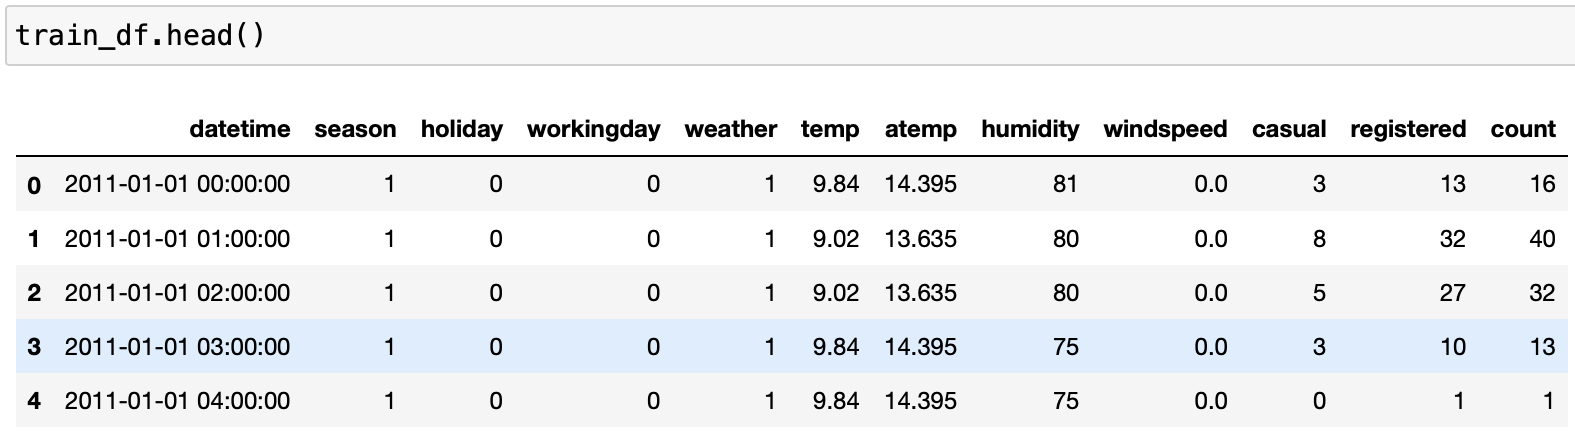
\includegraphics[width=0.8\textwidth,height=0.5\textwidth]{graphics/img/Data_summary1.eps}}
\end{figure}
\begin{figure}
  \centerline{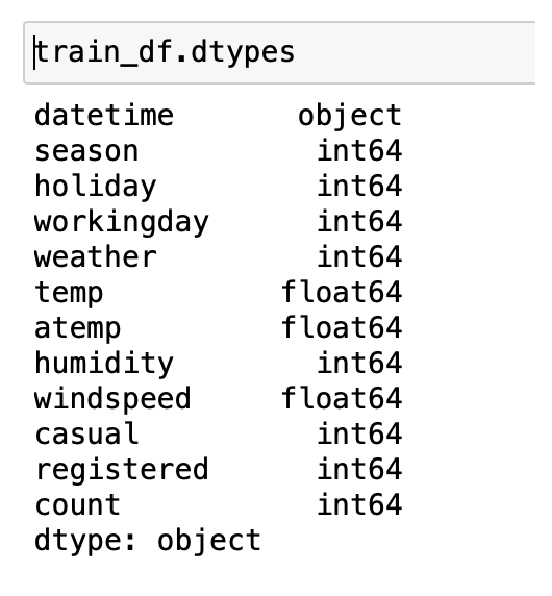
\includegraphics[width=0.4\textwidth,height=0.5\textwidth]{graphics/img/Data_summary2.eps}}
\end{figure}

\section{Correlation Matrix} \label{heatmap}
A common way to understand how target variables are affected by numerical features is to find the correlation matrix between them, plotting a heatmap of the correlation matrix between count and [temp, atemp, humidity, windspeed, casual, registered].\\
Based on the above heatmap, we can see that some of the features have no relation with the response variable. we can drop those columns.
\begin{itemize}
\item
\textcolor{orange} {humidity}, \textcolor{orange}{temp} are negatively correlated with count
\item
There is a strong correlation between \textcolor{orange} {temp} and \textcolor{orange} {atemp}, if both are included in the model, it will cause multicollinearity problems, so one of the features must be deleted. We remove the atemp feature because it has a weaker correlation with count than temp.
\item
\textcolor{orange} {Casual}, \textcolor{orange}{Registered} are not considered and removed during model building 
\item
\textcolor{orange} {humidity}, \textcolor{orange}{temp} and \textcolor{orange} {windspeed} features are considered during future modelling
\item 
fill in the zero values in the windspeed feature: usage is high when the wind speed is 0, which may be caused by null filling. Therefore, a random forest model is used here to fill in the zero values. 
\end{itemize}

\begin{figure}
  \centerline{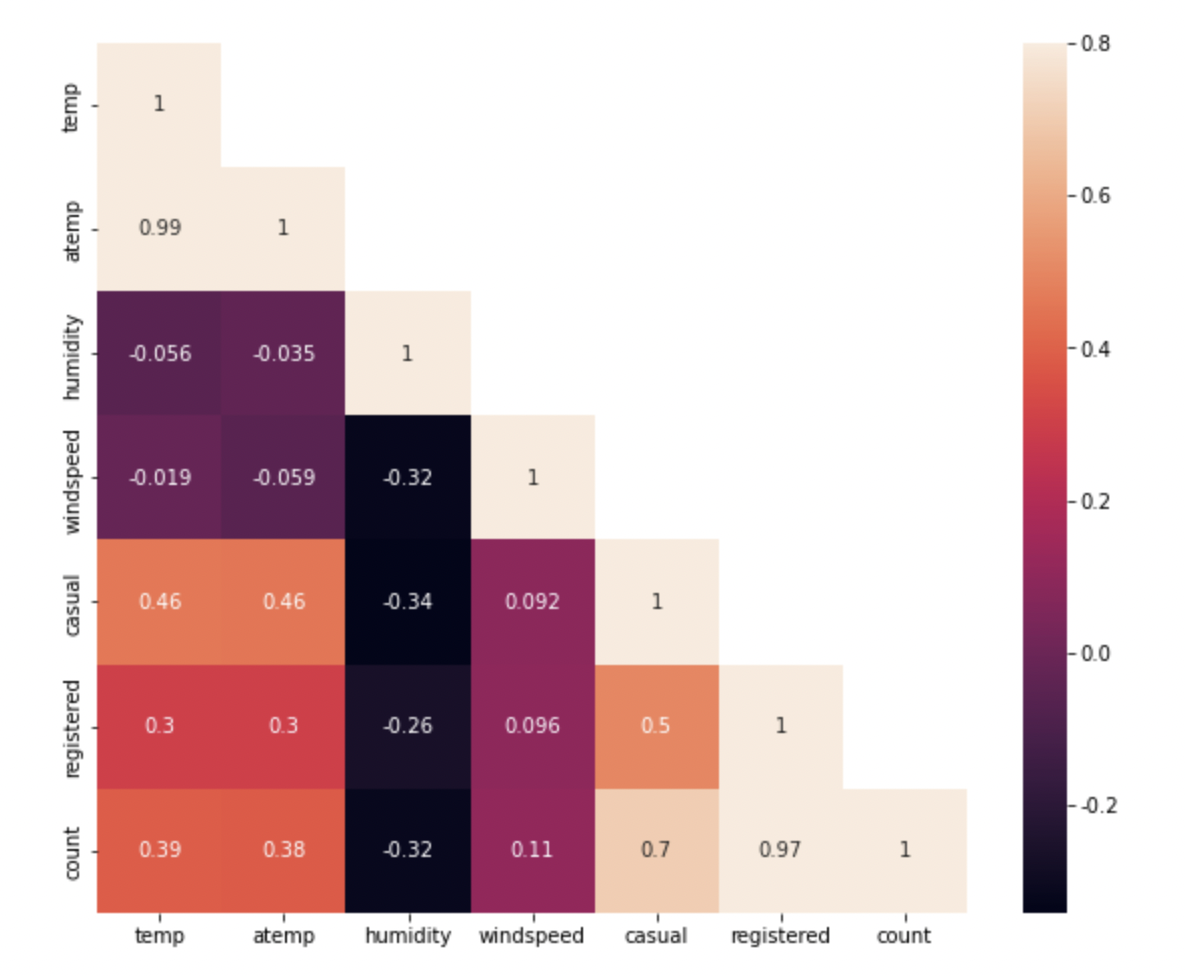
\includegraphics[width=0.6\textwidth,height=0.5\textwidth]{graphics/img/heatmap.eps}}
\end{figure}


% \section{Target variable Analysis} \label{target-variable}
%As can be seen from the figure below, the target variable count has a right-skewed distribution. Since most machine learning techniques require the dependent variable to be normally distributed, variable transformation is required. One possible solution is to log-transform the count variable after removing outlier data points. The transformed data looks much better, approximately following a normal distribution.

% \begin{figure}
%   \centerline{\includegraphics[width=0.6\textwidth,height=0.5\textwidth]{graphics/img/targetvariableanalysis.eps}}
% \end{figure}


\section{Predictive Modelling} \label{sec-model}
For the purpose of predictive modelling, the given dataset is divided into train set and test set.
\begin{itemize}
  \item Split the dataset into train set and test set
  \item Train Data size : 0.7
  \item Test Data size : 0.3
  \end{itemize}
Prediction with Linear Model
\begin{itemize}
  \item Linear Regression
  \item Ridge Regression
  \item Lasso Regression
  \item Logistic Regression
  \item ElasticNet
  \end{itemize}

  Prediction with Ensemble Learning Model
  \begin{itemize}
    \item Bagging Regressor
    \item Random Forest Regressor
    \item Gradient Boosting Regressor
    \item AdaBoost Regressor
    
    \end{itemize}

\section{Evaluation Results} \label{sec-result}
\begin{itemize}

  \item Evaluation Indicators: root mean square error is required (Root Mean Squared Logarithmic Error, RMSLE) to evaluate the quality of the model. 
  \smallskip
  
  {$$ RMSLE = \sqrt{\frac{1}{n} \sum_{i=1}^n [\log(p_i + 1) - \log(a_i + 1)]^2} $$}
  Among them, $n$ is the number of samples in the test set, $p_i$ is the test value, and $a_i$ is the actual value. The smaller the root mean square error, the better the fitting effect of the data, and the closer the test value is to the actual value.
  \end{itemize}

  \begin{table}[tb]
    \setlength{\abovecaptionskip}{0pt}
    \setlength{\belowcaptionskip}{10pt}
    \centering
    \caption{Model Evaluation Results}
    
    \begin{tabular}{ c | c | c | c }
    \toprule
      % after \\: \hline or \cline{col1-col2} \cline{col3-col4} ...
      Model     & Accuracy      \\
    \midrule
    Random Forest Regression        & 0.376319   \\
    Bagging Regression              & 0.395248    \\
    GBRT                            & 0.430378   \\
    AdaBoost Regression             & 0.703528   \\ 
    Ridge Regression                & 1.045335   \\
    Lasso Regression                & 1.045453 \\
    ElasticNet Regression           & 1.045489 \\
    Linear Regression               & 1.046341 \\
    Logistic Regression             & 1.131105 \\
    \bottomrule
    \end{tabular}
    \end{table}

\section{Conclusions} \label{sec-conclusions}

This is only the basic modeling of the data. The results can be further enhanced.

% \section*{Acknowledgement}

%\lipsum[1]


%The authors would like to thank \ldots



% ----------------------------------------------------------------
%\newpage
%\bibliographystyle{plain}
\bibliography{tuliplab,yourbib}
\bibliographystyle{IEEEtran}
%=================================================================

\listoftodos

\end{document}

